
\documentclass[11pt]{article}

\usepackage{graphicx}
\usepackage{float}
\usepackage{amssymb}
\usepackage{amsmath}
\usepackage{amsthm}
\usepackage{amsfonts}
\usepackage{enumitem}
\usepackage{pdfpages}
\usepackage[margin=1in]{geometry}

\newenvironment{solution}
  {\par\noindent\textbf{Solution:}\par}
  {\par}
\title{MATH 340, 2024/25, Term 2, Assignment 2}
\author{Mercury Mcindoe 85594505} 

\begin{document}
\maketitle 
\thispagestyle{empty}

\begin{enumerate}
  \item Consider the problem [Vanderbei 5th edition, Exercise 1.1].
    \begin{enumerate}[label=(\alph*)]
      \item Write this as a Linear Programming problem in the standard inequality form).
You must explain your notation and variables. 
      \begin{solution}
        Let's denote the variables for Bands and Coils as $x_b,x_c$ respectively. Then our goal is to 
        maximize $25x_b + 30x_c$ while satisfying the constraints  
        $$x_b \le 6000, x_c \le 4000, x_b \ge 0, x_c \ge 0, \frac{x_b}{200}+\frac{x_c}{140} \le 40$$

        Thus, we get the LP Problem in the standard inequality form,
        \[
        \begin{aligned}
          \text{maximize} \quad & 25x_b + 30x_c \\
          \text{subject to} \quad 
          & \frac{x_b}{200} + \frac{x_c}{140} \leq 40, \\
          & x_b \leq 6000, \\
          & x_c \leq 4000, \\
          & x_b, x_c \geq 0.
        \end{aligned}
\] 
      \end{solution}
     \item Solve the LP by writing down a code in the Python language using the Jupyter notebook; login to UBC syzygy website and the Jupyter notebook. Attach the pdf file that include both the code and the results; note that you can
save the Jupyter notebook as a pdf file. 
       \begin{solution}
      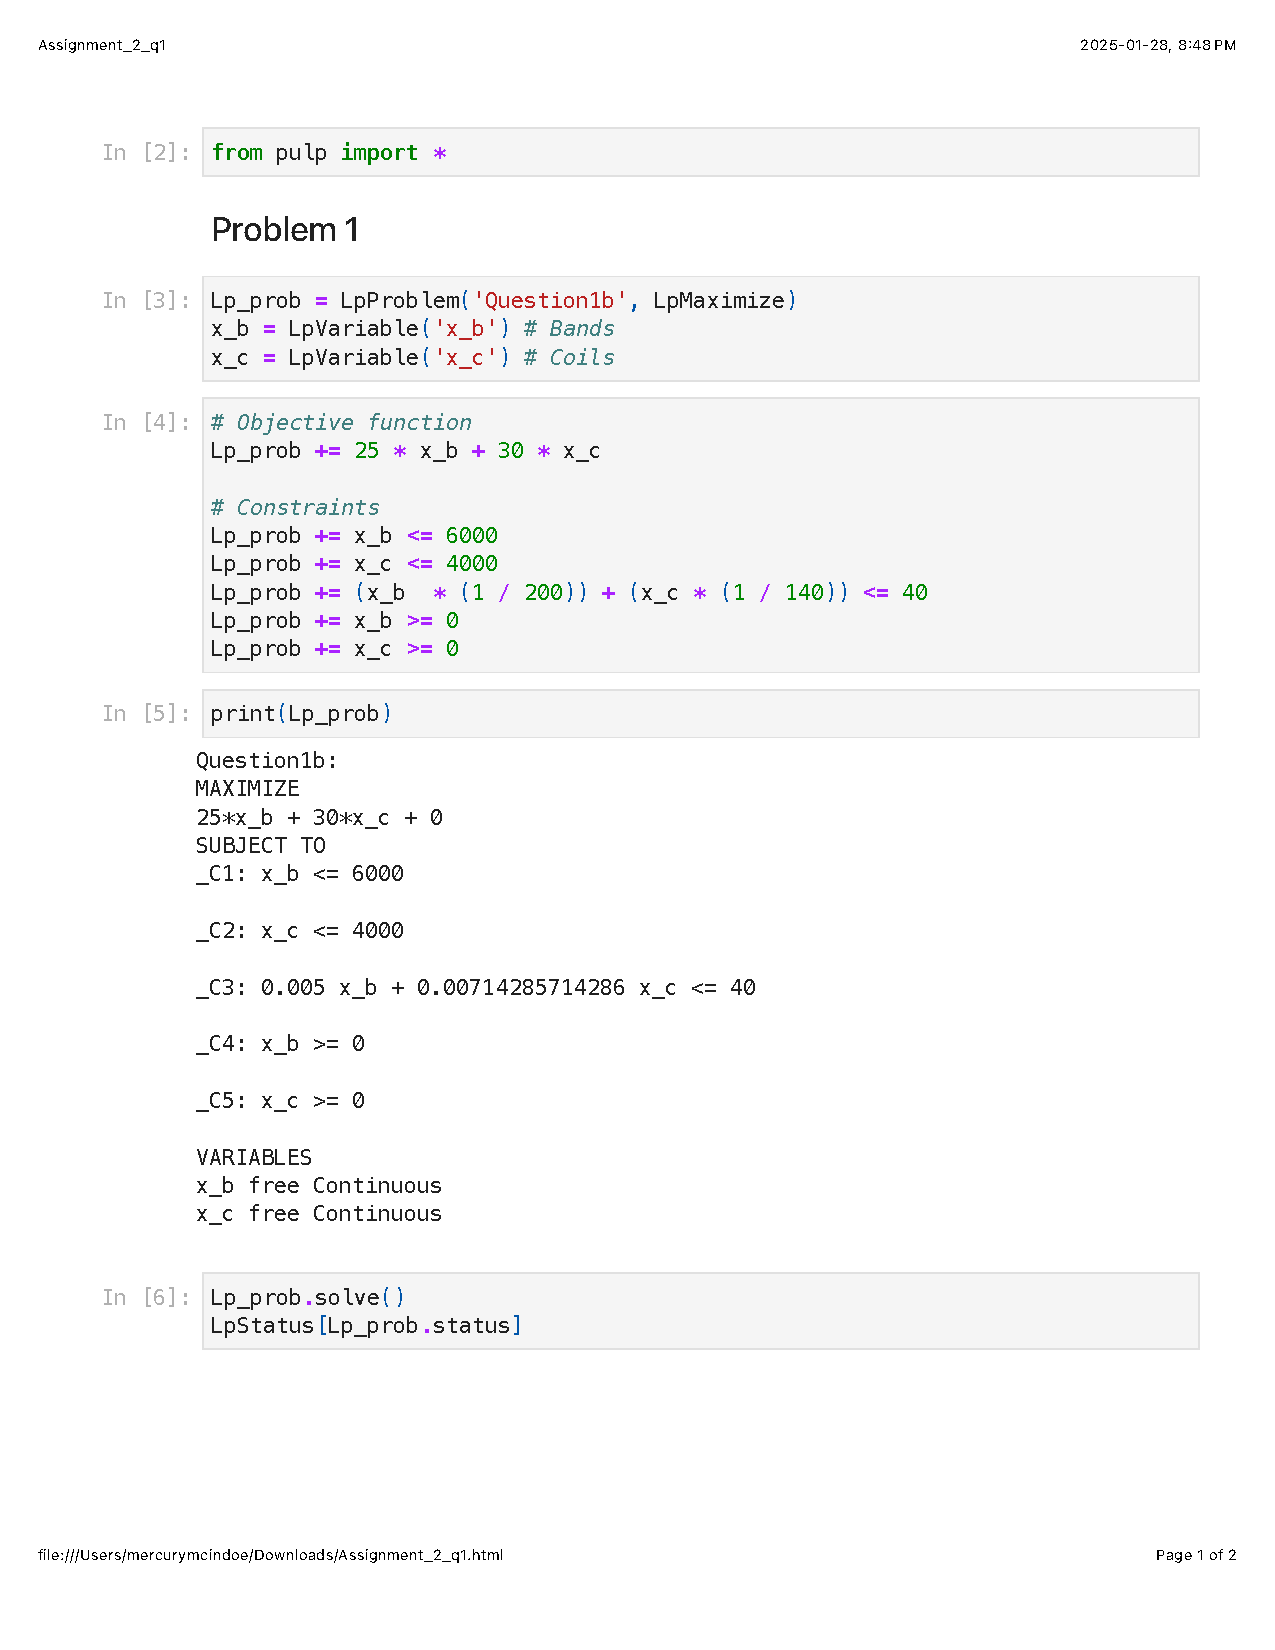
\includepdf[pages=-]{Assignment_2_q1.pdf}
       \end{solution}

\end{enumerate}
\item Consider the problem [Vanderbei. 5th edition, Exercise 1.2].
  \begin{enumerate}[label=(\alph*)]
    \item Write this as a Linear Programming problem (in the standard inequality form).
You must explain your notation and variables.
    \begin{solution}
      We denote the variables as the following: 
      \[
        \begin{aligned}
          x_\text{INY}:\quad & \text{Ithaca–Newark-Y}\\ 
          x_\text{INB}:\quad & \text{Ithaca–Newark-B}\\ 
          x_\text{INM}:\quad & \text{Ithaca–Newark-M}\\ 
          x_\text{NBY}:\quad & \text{Newark–Boston-Y}\\ 
          x_\text{NBB}:\quad & \text{Newark–Boston-B}\\ 
          x_\text{NBM}:\quad & \text{Newark–Boston-M}\\ 
          x_\text{IBY}:\quad & \text{Ithaca–Boston-Y}\\ 
          x_\text{IBB}:\quad & \text{Ithaca–Boston-B}\\ 
          x_\text{IBM}:\quad & \text{Ithaca–Boston-M}\\ 
        \end{aligned}
      \]
      The LP Problem is,
      \[
      \begin{aligned}
          \text{maximize} \quad &300  x_\text{INY}+ 220x_\text{INB} + 100  x_\text{INM} \\ 
                    & + 160 x_\text{NBY} + 130 x_\text{NBB}+ 80 x_\text{NBM} \\ 
                    & + 360  x_\text{IBY}+ 280 x_\text{IBB}+ 140 x_\text{IBM}\\
          \text{subject to} \quad 
          & x_\text{INY} \le 4 \\ 
          & x_\text{INB} \le 8 \\ 
          & x_\text{INM} \le 22 \\ 
          & x_\text{NBY} \le 8 \\ 
          & x_\text{NBB} \le 13 \\
          & x_\text{NBM} \le 20 \\ 
          & x_\text{IBY} \le 3 \\ 
          & x_\text{IBB} \le 10 \\ 
          & x_\text{IBM} \le 18\\
          & x_\text{INY} + x_\text{INB} + x_\text{INM} +  x_\text{IBY} +x_\text{IBB} + x_\text{IBM} \le 30\\        
          & x_\text{NBY} +  x_\text{NBB} + x_\text{NBM} + x_\text{IBY} + x_\text{IBB} + x_\text{IBM} \le 30 \\ 
          & x_\text{INY},x_\text{INB},x_\text{INM},x_\text{NBY},x_\text{NBB},x_\text{NBM} ,x_\text{IBY} ,x_\text{IBB} ,x_\text{IBM} \ge 0
        \end{aligned}
      \]

    \end{solution}
    \item Solve the LP by writing down a code in the Python language using the Jupyter
notebook; login to UBC syzygy website and the Jupyter notebook. Attach the pdf file that include both the code and the results; note that you can
save the Jupyter notebook as a pdf file. \\  Hint1: You will need integer variables, those taking only integer values. For that
you can add the command cat='Integer' like in the following example: \\ 
ticketvars = LpVariable.dicts("ticket", ticket, lowBound=0, cat='Integer') \\ 
Here the last part cat='Integer' restrict the variables to be integer variables. ] \\  Hint2: It is not necessary, but, to practice with 'for-loops' and 'dictionary', you
can try to use dictionary variables as done in the blending (cat food) example. ]
  \begin{solution}
    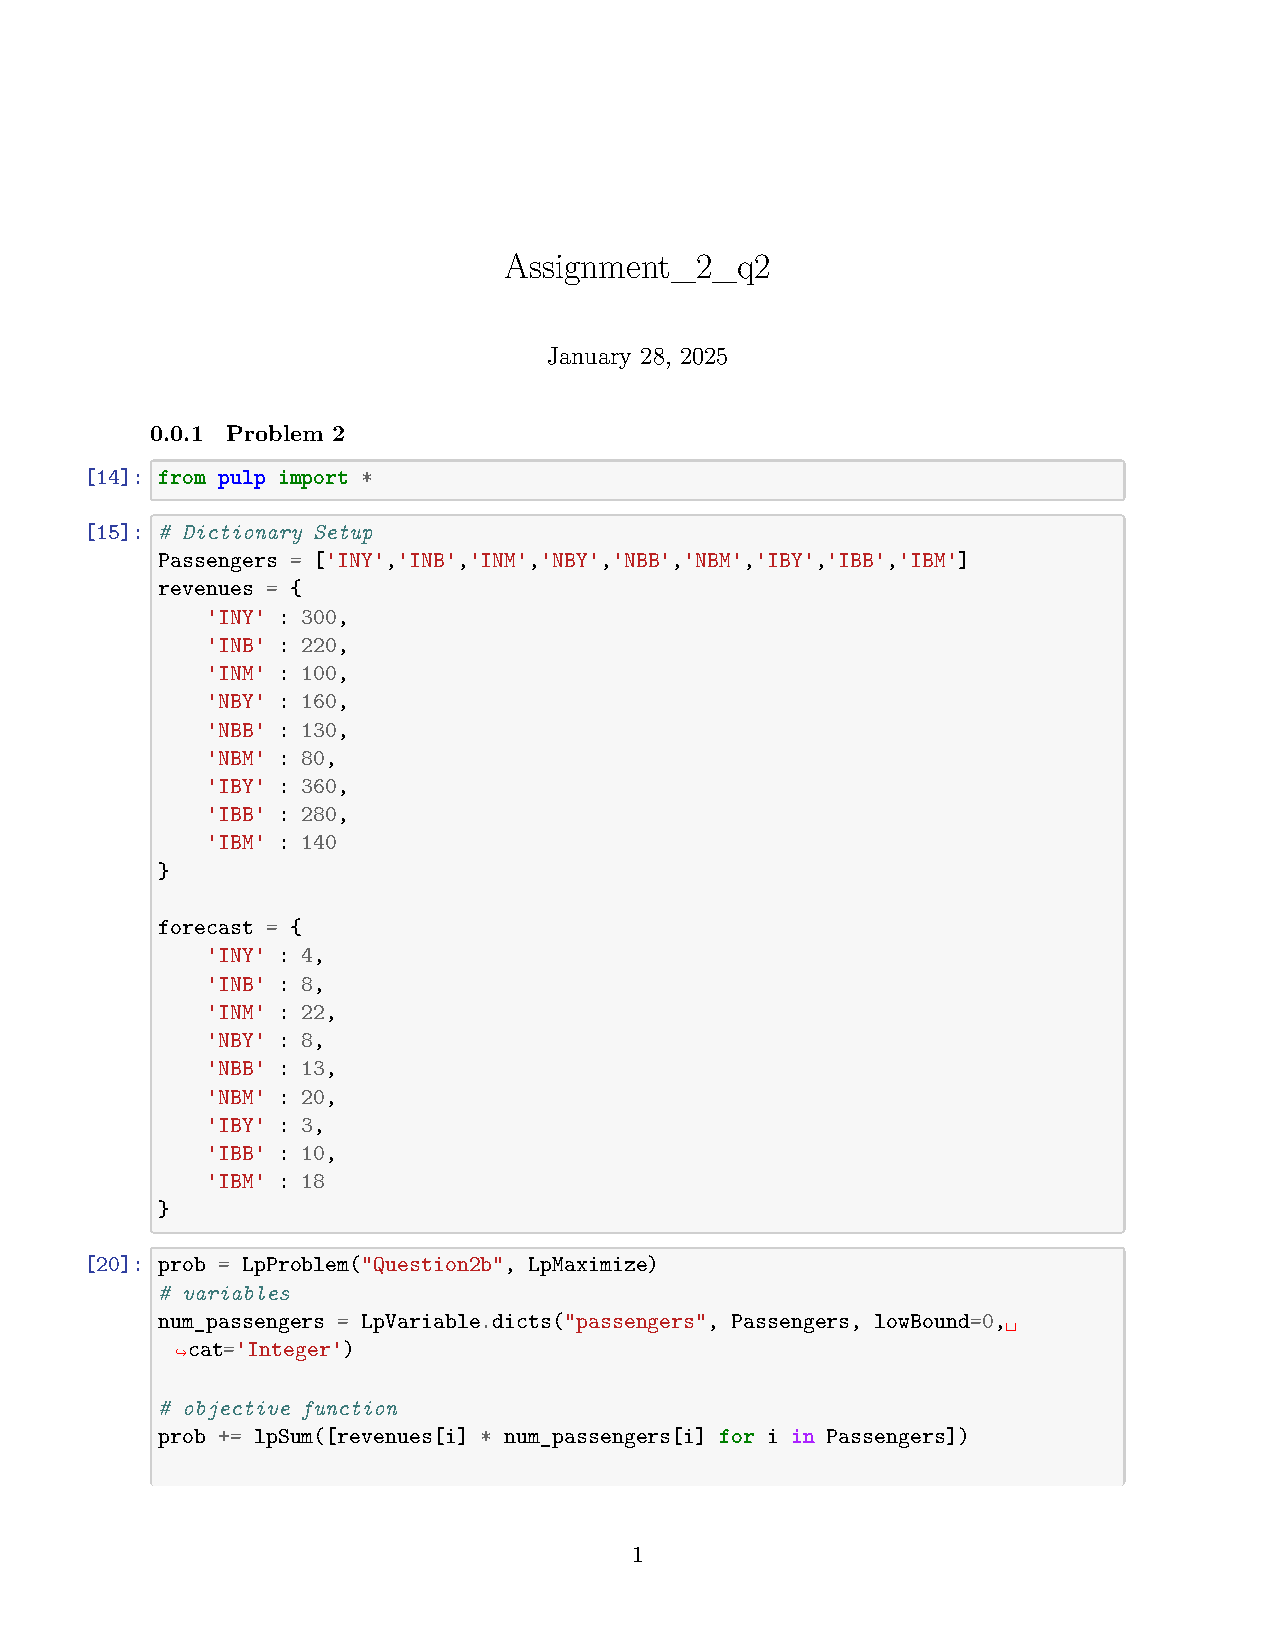
\includepdf[pages=-]{Assignment_2_q2.pdf}

  \end{solution}
  \end{enumerate}
  \item For a nonempty $S \subset \mathbf{R}^n$ and a positive real number $r \in \mathbb{R}$ (and $r > 0$),
    define the set $rS$ as follows:
    $$rS := \left\{ z \in \mathbf{R}^n \hspace{.05in} \vert \hspace{.05in} z = rx, x \in S \right\}$$
    Here $rx$ is the multiplication of the vector $x \in \mathbf{R}^n$ by the scalar $r \in \mathbf{R}$; in your more
    familiar notation, $r\vec{x}$. The set $rS$ is the set of all points that are obtained by multiplying
    $r$ with the vectors $x \in S$. \\ 
    For a given nonempty $S \subset \mathbf{R}^n$ and a given positive number $r>0$, prove that if $S$ is
    a convex set then $rS$ is a convex set as well.
    \begin{solution}
      Since $S$ is convex, for all $x, y \in S$ and $t \in [0,1]$, we have 
      $$(1-t)x + ty \in S.$$
      
      Let $w = (1-t)x + ty \in S$. For some $r \in \mathbf{R}^+$, we consider:
      $$rw = r(1-t)x + rty = (1-t)(rx) + t(ry).$$

      By the definition of $rS$, if $x, y, w \in S$, then $rx, ry, rw \in rS$. 

      Therefore, $rS$ is also a convex set.
    \end{solution}

  \item For given two nonempty sets $S_1,S_2 \subset \mathbf{R}^n$, define the operation $S_1+S_2$ as follows:
    $$S_1+S_2 := \left\{ z \in \mathbf{R}^n \hspace{.05in} \vert \hspace{.05in} \text{ there exist some } x \in S_1 \text{ and some } y \in S_2 \text{ such that } z =x+y \right\}$$
    that is, each point $z \in S_1 + S_2$ is the one that can be expressed as the sum $x+y$ for some $x \in S_1$,
    and $y \in S_2$; here the sum $x+y$ is the vector sum between the two vectors. One does this for 
    all $x \in S_1$ and $y \in S_2$ and get the set $S_1 + S_2$.

    \begin{enumerate}[label=(\alph*)]
      \item Consider $S_1 = \left\{ (x_1,x_2) \in \mathbf{R}^2 \hspace{.05in} \vert \hspace{.05in}
        \vert x_1 - 1\vert \le 1 \& \vert x_2 -2 \vert \le 1\right\}$ \\  
        and $ S_2 = \left\{ (x_1,x_2) \in \mathbf{R}^2 \hspace{.05in} \vert \hspace{.05in}
        \vert x_1\vert \le 2 \& \vert x_2 \vert \le 1\right\}$. Sketch the set $S_1 + S_2$. You do not need to explain 
        your solution for this question. But, your sketch should be neat and very clear, indicating all the 
        relevant coordinate values.
        \begin{solution}
        

\begin{figure}[H]
\centering
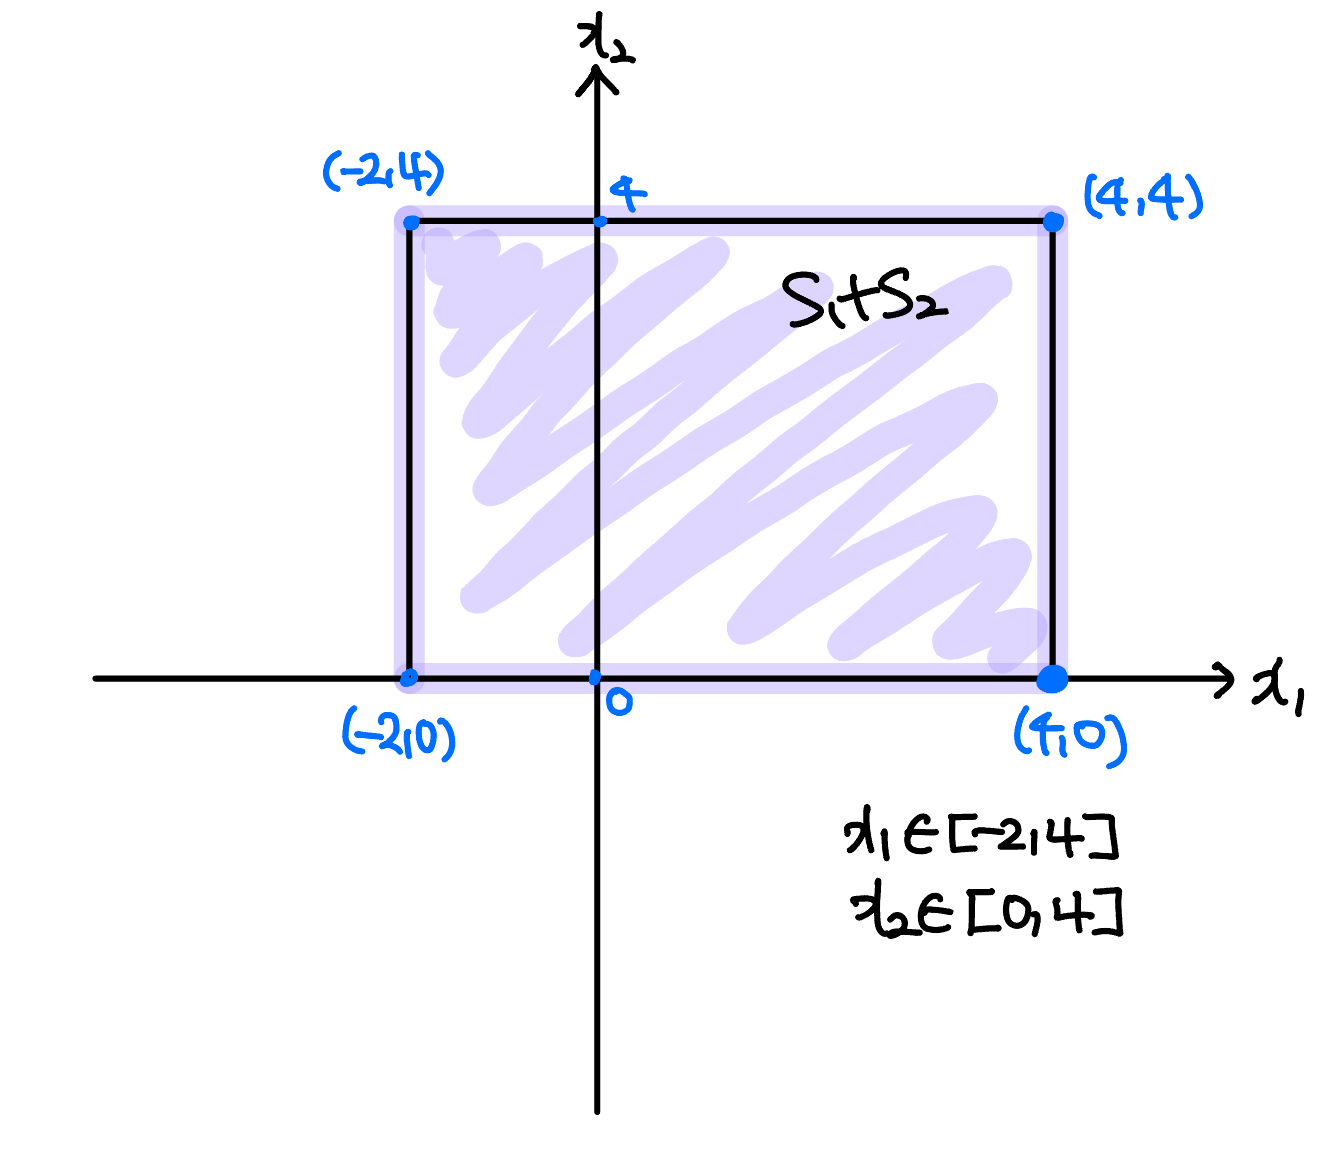
\includegraphics[width=0.6\textwidth]{figure1.png} 

\end{figure}


        \end{solution}
      \item Is it true that $S_1 + S_2$ must be convex for \textbf{any} nonempty convex sets $S_1$ and $S_2$ in
        $\mathbf{R}^n$? Justify your answer carefully. \textbf{[This problem is independent of part (a). 
        The sets $S_1,S_2$ are arbitrary convex sets in this question, not the particular example given in part (a).
        If you do this problem only for the sets of part (a) or a particular example, you will get zero mark.]}
        \begin{solution}
          Let $z_1,z_2 \in S_1 + S_2$ such that $z_1 = x_1 + y_1,z_2 = x_2 + y_2$ and $x_1,x_2 \in S_1$, $y_1,y_2 \in S_2$.
          First, let 
          \begin{align*}
            w &= w_1 + w_2 \\
              &= (1-t)z_1 + tz_2 \\
              &= (1-t)(x_1 + y_1) + t(x_2 + y_2) \\
              &= \{(1-t)x_1 + tx_2\} + \{(1-t)y_1 + ty_2\}.
          \end{align*}
          for some $t \in [0,1]$. \\ 
          Since $S_1$ and $S_2$ are non-empty convex sets, we have:
          \[
          w_1 = (1-t)x_1 + tx_2 \in S_1 \quad \text{and} \quad w_2 = (1-t)y_1 + ty_2 \in S_2.
          \]
          By the definition of $S_1 + S_2$, we can write:
          \[
          w = w_1 + w_2 = (1-t)z_1 + tz_2 \in S_1 + S_2, \quad t \in [0,1],
          \]
          proving that $S_1 + S_2$ is also a convex set.
      \end{solution}
    \end{enumerate}
\end{enumerate}
\end{document}
